\documentclass{standalone}
\usepackage{tikz}
\usetikzlibrary{patterns, positioning}
\usepackage[sfdefault]{ClearSans} %% option 'sfdefault' activates Clear Sans as the default text font
\usepackage[T1]{fontenc}

\begin{document}
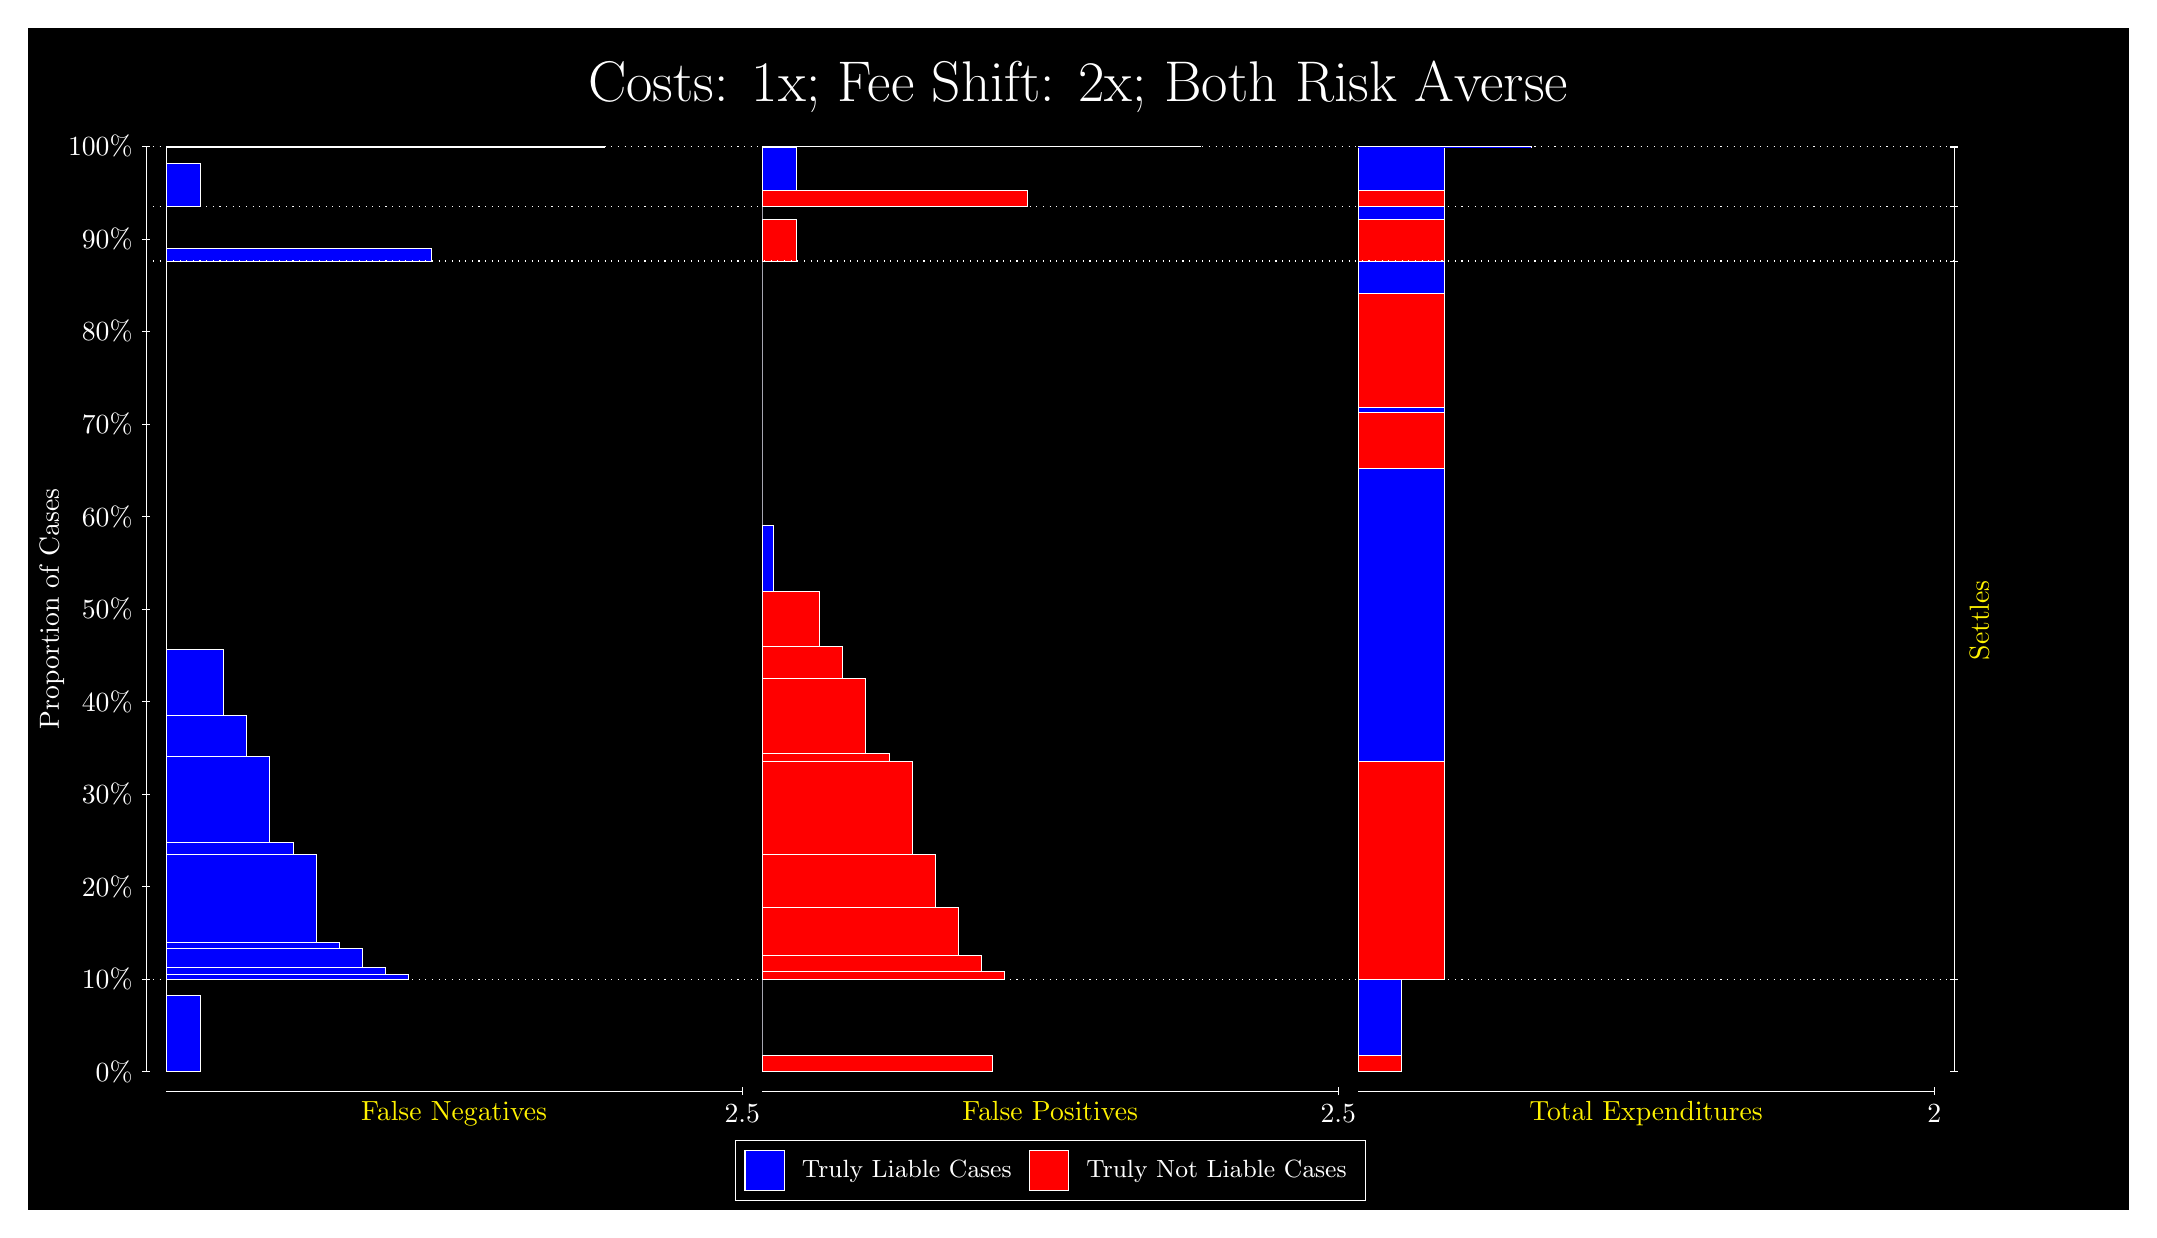
\begin{tikzpicture}
\draw[fill=black] (0,0) rectangle (26.667,15);
\draw[text=white] (0,13.5) rectangle (26.667,15) node[midway] {\huge Costs: 1x; Fee Shift: 2x; Both Risk Averse};
\draw[white, very thin] (1.5,1.75) -- (1.5,13.5);
\node[rotate=90, text=white, anchor=center] at (0.3, 7.625) {Proportion of Cases};
\draw[white, very thin] (1.45,1.75) -- (1.55,1.75);
\node[text=white, anchor=east] at (1.45, 1.75) {0\%};
\draw[white, very thin] (1.45,2.925) -- (1.55,2.925);
\node[text=white, anchor=east] at (1.45, 2.925) {10\%};
\draw[white, very thin] (1.45,4.1) -- (1.55,4.1);
\node[text=white, anchor=east] at (1.45, 4.1) {20\%};
\draw[white, very thin] (1.45,5.275) -- (1.55,5.275);
\node[text=white, anchor=east] at (1.45, 5.275) {30\%};
\draw[white, very thin] (1.45,6.45) -- (1.55,6.45);
\node[text=white, anchor=east] at (1.45, 6.45) {40\%};
\draw[white, very thin] (1.45,7.625) -- (1.55,7.625);
\node[text=white, anchor=east] at (1.45, 7.625) {50\%};
\draw[white, very thin] (1.45,8.8) -- (1.55,8.8);
\node[text=white, anchor=east] at (1.45, 8.8) {60\%};
\draw[white, very thin] (1.45,9.975) -- (1.55,9.975);
\node[text=white, anchor=east] at (1.45, 9.975) {70\%};
\draw[white, very thin] (1.45,11.15) -- (1.55,11.15);
\node[text=white, anchor=east] at (1.45, 11.15) {80\%};
\draw[white, very thin] (1.45,12.325) -- (1.55,12.325);
\node[text=white, anchor=east] at (1.45, 12.325) {90\%};
\draw[white, very thin] (1.45,13.5) -- (1.55,13.5);
\node[text=white, anchor=east] at (1.45, 13.5) {100\%};

\draw[white, very thin] (24.457,1.75) -- (24.457,13.5);
\draw[white, very thin] (24.407,1.75) -- (24.507,1.75);
\node[anchor=west] at (24.407, 1.75) {};
\draw[white, very thin] (24.407,2.9204) -- (24.507,2.9204);
\node[anchor=west] at (24.407, 2.9204) {};
\draw[white, very thin] (24.407,12.044) -- (24.507,12.044);
\node[anchor=west] at (24.407, 12.044) {};
\draw[white, very thin] (24.407,12.735) -- (24.507,12.735);
\node[anchor=west] at (24.407, 12.735) {};
\draw[white, very thin] (24.407,13.493) -- (24.507,13.493);
\node[anchor=west] at (24.407, 13.493) {};
\draw[white, very thin] (24.407,13.497) -- (24.507,13.497);
\node[anchor=west] at (24.407, 13.497) {};
\draw[white, very thin] (24.407,13.5) -- (24.507,13.5);
\node[anchor=west] at (24.407, 13.5) {};

\draw[white, very thin, fill=blue] (1.75,1.75) rectangle (2.1891,2.719);
\draw[white, very thin, fill=red] (1.75,2.719) rectangle (1.75,2.9204);
\draw[white, very thin, fill=blue] (1.75,2.9204) rectangle (4.8239,2.9818);
\draw[white, very thin, fill=blue] (1.75,2.9818) rectangle (4.5312,3.0693);
\draw[white, very thin, fill=blue] (1.75,3.0693) rectangle (4.2384,3.3194);
\draw[white, very thin, fill=blue] (1.75,3.3194) rectangle (3.9457,3.3875);
\draw[white, very thin, fill=blue] (1.75,3.3875) rectangle (3.6529,4.5031);
\draw[white, very thin, fill=blue] (1.75,4.5031) rectangle (3.3602,4.6673);
\draw[white, very thin, fill=blue] (1.75,4.6673) rectangle (3.0674,5.7561);
\draw[white, very thin, fill=blue] (1.75,5.7561) rectangle (2.7746,6.2775);
\draw[white, very thin, fill=blue] (1.75,6.2775) rectangle (2.4819,7.1106);
\draw[white, very thin, fill=red] (1.75,7.1106) rectangle (1.75,12.044);
\draw[white, very thin, fill=blue] (1.75,12.044) rectangle (5.1167,12.206);
\draw[white, very thin, fill=red] (1.75,12.206) rectangle (1.75,12.735);
\draw[white, very thin, fill=blue] (1.75,12.735) rectangle (2.1891,13.285);
\draw[white, very thin, fill=red] (1.75,13.285) rectangle (1.75,13.493);
\draw[white, very thin, fill=blue] (1.75,13.493) rectangle (7.3123,13.495);
\draw[white, very thin, fill=red] (1.75,13.495) rectangle (1.75,13.497);
\draw[white, very thin, fill=red] (1.75,13.497) rectangle (1.75,13.498);
\draw[white, very thin, fill=blue] (1.75,13.498) rectangle (1.75,13.5);
\draw[white, very thin, fill=red] (9.3189,1.75) rectangle (12.246,1.9515);
\draw[white, very thin, fill=blue] (9.3189,1.9515) rectangle (9.3189,2.9204);
\draw[white, very thin, fill=red] (9.3189,2.9204) rectangle (12.393,3.0239);
\draw[white, very thin, fill=red] (9.3189,3.0239) rectangle (12.1,3.2241);
\draw[white, very thin, fill=red] (9.3189,3.2241) rectangle (11.807,3.8414);
\draw[white, very thin, fill=red] (9.3189,3.8414) rectangle (11.515,4.5151);
\draw[white, very thin, fill=red] (9.3189,4.5151) rectangle (11.222,5.6936);
\draw[white, very thin, fill=red] (9.3189,5.6936) rectangle (10.929,5.7856);
\draw[white, very thin, fill=red] (9.3189,5.7856) rectangle (10.636,6.7491);
\draw[white, very thin, fill=red] (9.3189,6.7491) rectangle (10.344,7.15);
\draw[white, very thin, fill=red] (9.3189,7.15) rectangle (10.051,7.8537);
\draw[white, very thin, fill=blue] (9.3189,7.8537) rectangle (9.4652,8.6868);
\draw[white, very thin, fill=blue] (9.3189,8.6868) rectangle (9.3189,12.044);
\draw[white, very thin, fill=red] (9.3189,12.044) rectangle (9.758,12.573);
\draw[white, very thin, fill=blue] (9.3189,12.573) rectangle (9.3189,12.735);
\draw[white, very thin, fill=red] (9.3189,12.735) rectangle (12.686,12.943);
\draw[white, very thin, fill=blue] (9.3189,12.943) rectangle (9.758,13.493);
\draw[white, very thin, fill=red] (9.3189,13.493) rectangle (9.3189,13.496);
\draw[white, very thin, fill=blue] (9.3189,13.496) rectangle (9.3189,13.497);
\draw[white, very thin, fill=red] (9.3189,13.497) rectangle (14.881,13.498);
\draw[white, very thin, fill=blue] (9.3189,13.498) rectangle (11.954,13.5);
\draw[white, very thin, fill=red] (16.888,1.75) rectangle (17.437,1.9515);
\draw[white, very thin, fill=blue] (16.888,1.9515) rectangle (17.437,2.9204);
\draw[white, very thin, fill=red] (16.888,2.9204) rectangle (17.986,5.6936);
\draw[white, very thin, fill=blue] (16.888,5.6936) rectangle (17.986,9.4168);
\draw[white, very thin, fill=red] (16.888,9.4168) rectangle (17.986,10.12);
\draw[white, very thin, fill=blue] (16.888,10.12) rectangle (17.986,10.182);
\draw[white, very thin, fill=red] (16.888,10.182) rectangle (17.986,11.638);
\draw[white, very thin, fill=blue] (16.888,11.638) rectangle (17.986,12.044);
\draw[white, very thin, fill=red] (16.888,12.044) rectangle (17.986,12.573);
\draw[white, very thin, fill=blue] (16.888,12.573) rectangle (17.986,12.735);
\draw[white, very thin, fill=red] (16.888,12.735) rectangle (17.986,12.943);
\draw[white, very thin, fill=blue] (16.888,12.943) rectangle (17.986,13.493);
\draw[white, very thin, fill=red] (16.888,13.493) rectangle (19.083,13.496);
\draw[white, very thin, fill=blue] (16.888,13.496) rectangle (19.083,13.497);
\draw[white, very thin, fill=red] (16.888,13.497) rectangle (19.083,13.498);
\draw[white, very thin, fill=blue] (16.888,13.498) rectangle (19.083,13.5);
\draw[white, dotted] (1.5,2.9204) -- (24.457,2.9204);
\draw[white, dotted] (1.5,12.044) -- (24.457,12.044);
\draw[white, dotted] (1.5,12.735) -- (24.457,12.735);
\draw[white, dotted] (1.5,13.493) -- (24.457,13.493);
\draw[white, dotted] (1.5,13.497) -- (24.457,13.497);
\draw[white, very thin] (1.75,1.5) -- (9.0689,1.5);
\node[text=yellow, anchor=north] at (5.4094, 1.5) {False Negatives};
\draw[white, very thin] (9.0689,1.45) -- (9.0689,1.55);
\node[text=white, anchor=north] at (9.0689, 1.45) {2.5};

\draw[white, very thin] (9.3189,1.5) -- (16.638,1.5);
\node[text=yellow, anchor=north] at (12.978, 1.5) {False Positives};
\draw[white, very thin] (16.638,1.45) -- (16.638,1.55);
\node[text=white, anchor=north] at (16.638, 1.45) {2.5};

\draw[white, very thin] (16.888,1.5) -- (24.207,1.5);
\node[text=yellow, anchor=north] at (20.547, 1.5) {Total Expenditures};
\draw[white, very thin] (24.207,1.45) -- (24.207,1.55);
\node[text=white, anchor=north] at (24.207, 1.45) {2};


\node[text=yellow, centered, rotate=90] at (24.777, 7.4822) {Settles};





\draw (12.978300999999998,1.5) node[draw=none] (baseCoordinate) {};
\begin{scope}[align=center]
        \matrix[scale=0.5, draw=white, below=0.5cm of baseCoordinate, nodes={draw}, column sep=0.1cm]{
            \node[rectangle, draw, minimum width=0.5cm, minimum height=0.5cm, fill=blue] {}; &
            \node[draw=none, font=\small, text=white] (B) {Truly Liable Cases}; &
            \node[rectangle, draw, minimum width=0.5cm, minimum height=0.5cm, fill=red] {}; &
            \node[draw=none, font=\small, text=white] (B) {Truly Not Liable Cases}; \\
            };
\end{scope}

\end{tikzpicture}
\end{document}